\documentclass{standalone}
\usepackage{tikz}\usepackage{graphicx}

\usetikzlibrary{shapes,arrows}
\usetikzlibrary{shapes.geometric,positioning}


\begin{document}
    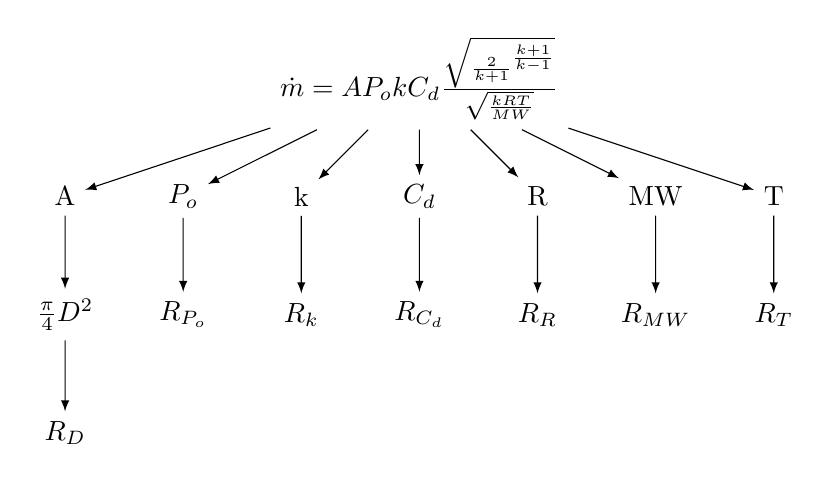
\begin{tikzpicture}[edge from parent/.style={-latex, draw=black}]
        \node (a) at (0,0) [above]  {$\dot{m} = AP_{o}k C_{d} \frac{\sqrt{\frac{2}{k+1}^{\frac{k+1}{k-1}}}}{\sqrt{\frac{kRT}{MW}}}$} 
        child{node{A}
            child{node{$\frac{\pi}{4}D^{2}$}
                child{node{$R_{D}$}}}}
        child{node{$P_{o}$}
            child{node{$R_{P_{o}}$}}}
        child{node{k}
            child{node{$R_{k}$}}}
        child{node{$C_{d}$}
            child{node{$R_{C_{d}}$}}}
        child{node{R}
            child{node{$R_{R}$}}}
        child{node{MW}
            child{node{$R_{MW}$}}}
        child{node{T}
            child{node{$R_{T}$}}}
            ;
    \end{tikzpicture}
\end{document}